\documentclass{article}
\usepackage[paperwidth=17cm,paperheight=8cm,margin=0pt]{geometry}
\usepackage{fontspec,tikz}
\usepackage[table]{xcolor}
\usetikzlibrary{arrows.meta}
\IfFontExistsTF{Helvetica Neue}
  {\setmainfont{Helvetica Neue}\setsansfont{Helvetica Neue}}
  {\IfFontExistsTF{Arial}{\setmainfont{Arial}\setsansfont{Arial}}{}}
\definecolor{navy}{HTML}{315E75}
\definecolor{teal}{HTML}{2E766E}
\definecolor{amber}{HTML}{A17431}
\definecolor{lightblue}{HTML}{EAF3F7}
\definecolor{mediumblue}{HTML}{9CC0D1}
\definecolor{lightteal}{HTML}{EDF6F2}
\definecolor{lightamber}{HTML}{FAF3E5}
\definecolor{lightrow}{HTML}{F7FAFB}
\definecolor{hairline}{HTML}{BDD0D8}
\pagestyle{empty}
\begin{document}
% Mirrors section 7 of the written outline: Home leads with analytics and the
% assistant entry; the assistant panel is expanded; Forum and Game are previewed
% as supporting tabs rather than given a screen each.
\noindent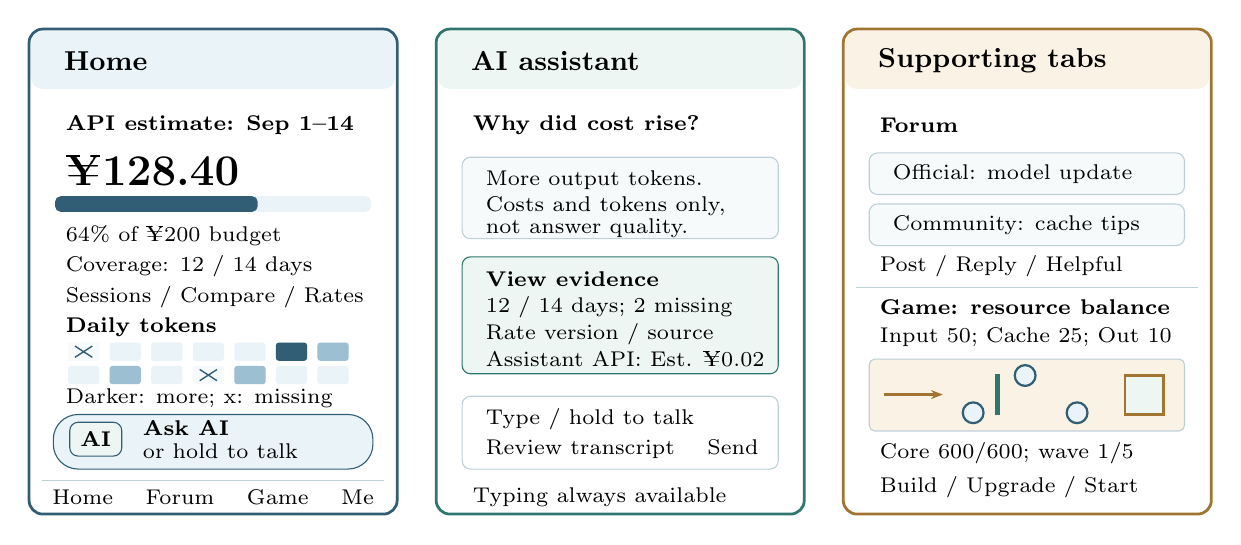
\begin{tikzpicture}[scale=1.1,transform shape,font=\scriptsize,every node/.style={text=black}]
\foreach \x/\title/\border/\filltone in {0/Home/navy/lightblue,4.7/AI assistant/teal/lightteal,9.4/Supporting tabs/amber/lightamber}{
  \draw[draw=\border,line width=1pt,rounded corners=5pt] (\x,0) rectangle (\x+4.25,5.6);
  \fill[\filltone,rounded corners=4pt] (\x+.025,4.91) rectangle (\x+4.225,5.575);
  \node[anchor=west,font=\small\bfseries] at (\x+.28,5.23) {\title};
}
% Home: cost and budget lead; a neutral AI icon anchors the floating entry.
\node[anchor=west,font=\scriptsize\bfseries] at (.3,4.49) {API estimate: Sep 1--14};
\node[anchor=west,font=\Large\bfseries] at (.3,3.97) {¥128.40};
\fill[lightblue,rounded corners=2pt] (.3,3.49) rectangle (3.95,3.67);
\fill[navy,rounded corners=2pt] (.3,3.49) rectangle (2.64,3.67);
\node[anchor=west] at (.3,3.22) {64\% of ¥200 budget};
\node[anchor=west] at (.3,2.86) {Coverage: 12 / 14 days};
\node[anchor=west] at (.3,2.50) {Sessions / Compare / Rates};
\node[anchor=west,font=\scriptsize\bfseries] at (.3,2.16) {Daily tokens};
\foreach \col in {0,...,6}{\foreach \row in {0,...,1}{\fill[lightblue,rounded corners=1pt] ({.45+.48*\col},{1.50+.27*\row}) rectangle ({.81+.48*\col},{1.71+.27*\row});}}
\foreach \col/\row/\tone in {1/0/mediumblue,2/1/lightblue,4/0/mediumblue,5/1/navy,6/1/mediumblue}{\fill[\tone,rounded corners=1pt] ({.45+.48*\col},{1.50+.27*\row}) rectangle ({.81+.48*\col},{1.71+.27*\row});}
\foreach \col/\row in {0/1,3/0}{\fill[lightrow] ({.45+.48*\col},{1.50+.27*\row}) rectangle ({.81+.48*\col},{1.71+.27*\row});\draw[navy,line width=.5pt] ({.53+.48*\col},{1.54+.27*\row}) -- ({.73+.48*\col},{1.67+.27*\row}) ({.53+.48*\col},{1.67+.27*\row}) -- ({.73+.48*\col},{1.54+.27*\row});}
\node[anchor=west] at (.3,1.34) {Darker: more; x: missing};
\draw[draw=navy,fill=lightblue,rounded corners=9pt] (.28,.52) rectangle (3.97,1.15);
\draw[draw=navy,fill=lightteal,rounded corners=3pt] (.47,.67) rectangle (1.07,1.06);
\node[font=\scriptsize\bfseries] at (.77,.865) {AI};
\node[anchor=west,font=\scriptsize\bfseries] at (1.19,.99) {Ask AI};
\node[anchor=west] at (1.19,.73) {or hold to talk};
\draw[hairline] (.15,.39) -- (4.10,.39);
\node at (2.125,.19) {Home \quad Forum \quad Game \quad Me};
% Expanded assistant panel: question, traceable evidence and separate model cost.
\node[anchor=west,font=\scriptsize\bfseries] at (5.0,4.49) {Why did cost rise?};
\draw[draw=hairline,fill=lightrow,rounded corners=3pt] (5.0,3.18) rectangle (8.65,4.12);
\node[anchor=west] at (5.15,3.86) {More output tokens.};
\node[anchor=west] at (5.15,3.55) {Costs and tokens only,};
\node[anchor=west] at (5.15,3.30) {not answer quality.};
\draw[draw=teal,fill=lightteal,rounded corners=3pt] (5.0,1.62) rectangle (8.65,2.97);
\node[anchor=west,font=\scriptsize\bfseries] at (5.15,2.71) {View evidence};
\node[anchor=west] at (5.15,2.39) {12 / 14 days; 2 missing};
\node[anchor=west] at (5.15,2.08) {Rate version / source};
\node[anchor=west] at (5.15,1.79) {Assistant API: Est. ¥0.02};
\draw[draw=hairline,rounded corners=3pt] (5.0,.52) rectangle (8.65,1.36);
\node[anchor=west] at (5.15,1.10) {Type / hold to talk};
\node[anchor=west] at (5.15,.75) {Review transcript \quad Send};
\node[anchor=west] at (5.0,.20) {Typing always available};
% Two compact previews show the supporting tabs without displacing the core screens.
\node[anchor=west,font=\scriptsize\bfseries] at (9.7,4.49) {Forum};
\draw[draw=hairline,fill=lightrow,rounded corners=3pt] (9.7,3.69) rectangle (13.34,4.17);
\node[anchor=west] at (9.85,3.93) {Official: model update};
\draw[draw=hairline,fill=lightrow,rounded corners=3pt] (9.7,3.10) rectangle (13.34,3.58);
\node[anchor=west] at (9.85,3.34) {Community: cache tips};
\node[anchor=west] at (9.7,2.86) {Post / Reply / Helpful};
\draw[hairline] (9.55,2.62) -- (13.50,2.62);
\node[anchor=west,font=\scriptsize\bfseries] at (9.7,2.39) {Game: resource balance};
\node[anchor=west] at (9.7,2.04) {Input 50; Cache 25; Out 10};
\draw[draw=hairline,fill=lightamber,rounded corners=2pt] (9.7,.96) rectangle (13.34,1.79);
\draw[-{Stealth[length=1.5mm]},draw=amber,line width=.8pt] (9.87,1.38) -- (10.55,1.38);
\foreach \x/\y in {10.9/1.17,11.5/1.60,12.1/1.17}{\draw[draw=navy,fill=lightblue,line width=.8pt] (\x,\y) circle (.12);}
\draw[draw=teal,line width=2pt] (11.18,1.14) -- (11.18,1.62);
\draw[draw=amber,fill=lightteal,line width=.9pt] (12.65,1.15) rectangle (13.10,1.60);
\node[anchor=west] at (9.7,.70) {Core 600/600; wave 1/5};
\node[anchor=west] at (9.7,.31) {Build / Upgrade / Start};
\end{tikzpicture}
\end{document}
